\section{Introduction}

\begin{frame}{Introduction}
An \emph{intersection graph} is a graph $G = (\zeta, E)$ where $\zeta$ is a collection of objects. Two vertices of the graph are adjacent if the objects \emph{intersect}.

\vfill
\pause

\begin{columns}
  \begin{column}{0.5\textwidth}

    \begin{figure}
    \begin{center}
    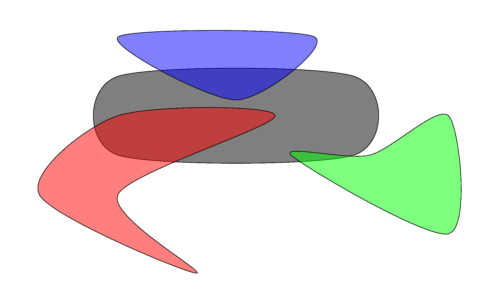
\begin{tikzpicture}[scale=1]
    \def\ver{0.1} %size of a vertex
    \def\x{1}

    \def\xa{0.5}
    \def\ya{0}

    \def\xd{4.5}
    \def\yd{0}

    \draw [fill=black, opacity= 0.5] plot [smooth cycle] coordinates {(0,1.5) (0,0.5) (3,0.5) (3,1.5)};

    \draw [fill=red, opacity=0.5] plot [smooth cycle] coordinates {(-1,0) (0,1) (2,1) (0,0) (1,-1)};

    \draw [fill=green, opacity= 0.5] plot [smooth cycle] coordinates {(2.2,0.5) (3.2,0.5) (4.2,1) (4.2,-0.5)};

    \draw [fill=blue, opacity= 0.5] plot [smooth cycle] coordinates {(1.5,1.2) (0,2) (2.5,2)};


    \end{tikzpicture}
    \end{center}
    \end{figure}
  \pause
  \end{column}
  \begin{column}{0.5\textwidth}
    \begin{figure}
    \begin{center}
      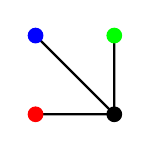
\begin{tikzpicture}[scale=1]
    \def\ver{0.1} %size of a vertex
    \def\x{1}

    \def\xa{0.5}
    \def\ya{0}

    \def\xd{4.5}
    \def\yd{0}


    \draw[thick] (\xa,\ya)--(\xa+1,\ya)--(\xa+1,\ya+1) (\xa, \ya+1) -- (\xa +1, \ya);

    %graph R_0
    \path[fill=red] (\xa,\ya) circle (\ver);
    \path[fill=green] (\xa+1,\ya+1) circle (\ver);
    \path[fill=blue] (\xa,\ya+1) circle (\ver);
    \path[fill] (\xa+1,\ya) circle (\ver);


    \end{tikzpicture}
    \end{center}
    \end{figure}

  \end{column}
\end{columns}
\end{frame}


\begin{frame}{Introduction}
A \emph{forbidden subgraph/minor characterization} is a description of a family of graphs based on the graphs that do not belong to that family.
\vfill
\pause

\begin{example}[Kuratowski]
  A graph $G$ is planar if it does not contain $K_{3,3}$ or $K_5$ as a minor.
\end{example}
\end{frame}
